\documentclass[11pt]{article}

\hoffset        2mm 
\voffset        -15mm
\oddsidemargin  0mm
\topmargin      0.35in
\textwidth      6in
\textheight     9in

%\usepackage[parfill]{parskip}
\usepackage{graphicx}
\usepackage{amsmath}
\usepackage{mathtools}
\usepackage{booktabs}
\usepackage{enumerate}
\usepackage{listings}
\usepackage{float}
\usepackage{epstopdf}

\begin{document}


\begin{center}
{\em \huge Higher-Order FEM Basis Functions on Triangular Prisms}\\[8mm]
{\LARGE By: Michael Hackemack}\\[3mm]
{\large July 9, 2016} \\[15mm]
\end{center}



%%%%%%%%%%%%%%%%%%%%%%%%%%%%%%%%%%%%%%%%%%%%%%%%%%%%%%%%%%%%%%%%%%%%%%
%%%%%%%%%%%%%%%%%%%%%%%%%%%%%%%%%%%%%%%%%%%%%%%%%%%%%%%%%%%%%%%%%%%%%%
\section{Introduction}
\label{sec::Introduction}

In this document, we derive 

%%%%%%%%%%%%%%%%%%%%%%%%%%%%%%%%%%%%%%%%%%%%%%%%%%%%%%%%%%%%%%%%%%%%%%
%%%%%%%%%%%%%%%%%%%%%%%%%%%%%%%%%%%%%%%%%%%%%%%%%%%%%%%%%%%%%%%%%%%%%%
\section{Reference Basis Functions on a Triangle}
\label{sec::triref}

%%%%%%%%%%%%%%%%%%
%%%%%%%%%%%%%%%%%%
\subsection{Linear Basis Functions on the Reference Triangle}
\label{sec::triref_linear}




%%%%%%%%%%%%%%%%%%
%%%%%%%%%%%%%%%%%%
\subsection{Quadratic Basis Functions on the Reference Triangle}
\label{sec::triref_quadratic}


\begin{figure}[hbt]
\centering
	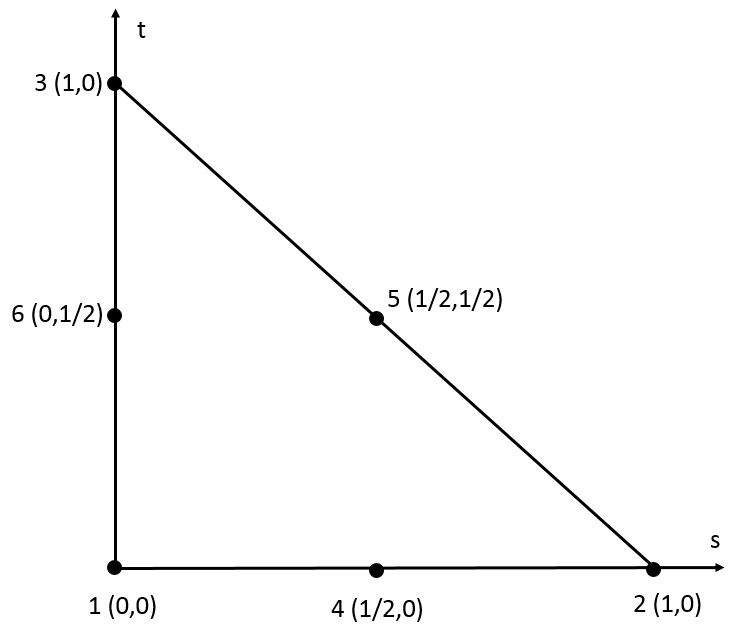
\includegraphics[width=3.0in]{./Figures/ref_triangle.jpg}
	\caption{Reference Triangle.}
\hspace{0.5cm}
\label{fig::ref_triangle}
\end{figure}

For this work, we choose the standard quadratic shape functions for triangles. The value and gradient equations for the basis functions on the reference triangle are given in Eq. (\ref{eq::basis_vals}).

\begin{equation}
	\begin{aligned}
		b_1(s,t) \, =& \, (1-s-t) (1-2s-2t),  &\vec{\nabla}& b_1(s,t) \, = \, \left( 4(s+t)-1 , 4(s+t)-1   \right) \\
		b_2(s,t) \, =& \, 2s(s-1/2),             &\vec{\nabla}& b_2(s,t) \, = \, \left( 4s-1, 0   \right) \\
		b_3(s,t) \, =& \, 2t(t-1/2),              &\vec{\nabla}& b_3(s,t) \, = \, \left( 0, 4t-1   \right) \\
		b_4(s,t) \, =& \, 4s (1-s-t),             &\vec{\nabla}& b_4(s,t) \, = \, \left( 4-8s, -4s   \right) \\
		b_5(s,t) \, =& \, 4st,                       &\vec{\nabla}& b_5(s,t) \, = \, \left( 4t, 4s   \right) \\
		b_6(s,t) \, =& \, 4t (1-s-t),             &\vec{\nabla}& b_6(s,t) \, = \, \left( -4t, 4-8t   \right) 
	\end{aligned}
\label{eq::basis_vals}
\end{equation}

%%%%%%%%%%%%%%%%%%
%%%%%%%%%%%%%%%%%%
\subsection{Cubic Basis Functions on the Reference Triangle}
\label{sec::triref_cubic}

%%%%%%%%%%%%%%%%%%
%%%%%%%%%%%%%%%%%%
\subsection{Quartic Basis Functions on the Reference Triangle}
\label{sec::triref_quartic}

%%%%%%%%%%%%%%%%%%%%%%%%%%%%%%%%%%%%%%%%%%%%%%%%%%%%%%%%%%%%%%%%%%%%%%
%%%%%%%%%%%%%%%%%%%%%%%%%%%%%%%%%%%%%%%%%%%%%%%%%%%%%%%%%%%%%%%%%%%%%%
\section{Reference Basis Functions on a Triangular Prism}
\label{sec::triprismref}

%%%%%%%%%%%%%%%%%%%%%%%%%%%%%%%%%%%%%%%%%%%%%%%%%%%%%%%%%%%%%%%%%%%%%%
%%%%%%%%%%%%%%%%%%%%%%%%%%%%%%%%%%%%%%%%%%%%%%%%%%%%%%%%%%%%%%%%%%%%%%
\section{Computing the Jacobian Transformation}
\label{sec::jacobian}


%%%%%%%%%%%%%%%%%%%%%%%%%%%%%%%%%%%%%%%%%%%%%%%%%%%%%%%%%%%%%%%%%%%%%%
%%%%%%%%%%%%%%%%%%%%%%%%%%%%%%%%%%%%%%%%%%%%%%%%%%%%%%%%%%%%%%%%%%%%%%
\section{Conclusions}
\label{sec::conclusions}

%%%%%%%%%%%%%%%%%%%%%%%%%%%%%%%%%%%%%%%%%%%%%%%%%%%%%%%%%%%%%%%%%%%%%%
%%%%%%%%%%%%%%%%%%%%%%%%%%%%%%%%%%%%%%%%%%%%%%%%%%%%%%%%%%%%%%%%%%%%%%
\section{References}
\label{sec::references}

\bibliographystyle{ans}
\bibliography{references}


\end{document}


